\chapter{Introdución}

O obxectivo principal deste traballo é o deseño e desenvolvemento de \textbf{Telaria},
unha aplicación móbil colaborativa para a xestión integral de viaxes en grupo. A idea
de partida é sinxela: ofrecer un \textit{espazo de viaxe} único e compartido no que un
grupo de persoas poida organizar todo o ciclo de vida dunha viaxe (antes, durante e despois) sen
ter que interactuar con media ducia de aplicacións xenéricas non pensadas para ese fin.

\section{Motivación e contexto}

A organización dunha viaxe en grupo é, na práctica, un problema de coordinación entre
varias persoas que comparten un mesmo obxectivo pero usan ferramentas distintas e
illadas entre si. Durante a fase de planificación adóitanse acumular as reservas de
aloxamento e transporte no correo ou na galería de cada quen, os horarios nun calendario
persoal e as propostas de actividades nun grupo de mensaxería. Xa durante a viaxe,
súmanse a ese caos os tíckets dos gastos compartidos e as fotos dos documentos
importantes. Ningunha desas ferramentas foi concibida para o contexto concreto dunha
viaxe, polo que a información queda repartida e desactualizada.

Esta fragmentación tradúcese en custos reais para o grupo. O máis evidente é o
económico: ao final da viaxe ninguén sabe con certeza canto puxo cada persoa nin como
saldar as contas, e a liquidación faise a man, de forma propensa a erros e a
transferencias innecesarias. A iso engádese a perda de información (un billete esquecido
no fondo dun fío de chat de centos de mensaxes), a dependencia dunha única persoa que «leva» a
organización e a dificultade de que todos os participantes teñan unha visión completa e
actualizada do plan.

A utilidade que persigue Telaria é precisamente eliminar ese traballo de
coordinación manual. Ao reunir gastos, calendario, documentos, comunicación e asistencia
intelixente nun mesmo espazo compartido por viaxe, cada participante accede sempre á
mesma información actualizada e o esforzo de mantela sincronizada desaparece. O público
ao que se dirixe non é o da viaxe corporativa nin o das axencias, senón os grupos
informais (cuadrillas de amizades, familias ou compañeiros) que viaxan xuntos de cando
en vez e que hoxe resolven esta coordinación cun conxunto disperso de aplicacións
xenéricas.

\section{Solucións existentes e diferenciación}

No mercado existen aplicacións que cobren \textit{partes} do problema descrito, pero
ningunha o aborda de forma integrada para o contexto dunha viaxe en grupo. As
alternativas máis representativas son as seguintes:

\begin{itemize}
  \item \textbf{Tricount}~\cite{tricount}: especializada na xestión de gastos
        compartidos e no cálculo de quen debe a quen. Resolve ben a parte económica, pero
        non ofrece calendario, almacenamento de documentos, chat de grupo nin asistencia
        intelixente. Foi, de feito, unha das inspiracións do proxecto: o seu enfoque da
        liquidación de gastos é o punto de partida que Telaria estende ao resto de
        necesidades dunha viaxe.
  \item \textbf{WhatsApp e grupos de mensaxería}~\cite{whatsapp}: cobren a comunicación
        do grupo, que é onde acaba converxendo o resto da organización por falta dun lugar
        mellor. Todo o demais (gastos, calendario, documentos) queda como información non
        estruturada dentro do fío de conversa, sen ningún tratamento específico.
  \item \textbf{Google Calendar}~\cite{googlecalendar}: resolve a planificación temporal,
        pero é unha ferramenta de calendario xenérica e centrada no individuo, non un
        espazo colaborativo organizado por viaxe nin integrado co resto de necesidades.
  \item \textbf{Wanderlog e TravelPerk}~\cite{wanderlog,travelperk}: son planificadores
        de viaxe máis completos, pero orientados respectivamente ao descubrimento de
        itinerarios e á xestión de viaxes corporativas. Teñen un soporte feble da
        liquidación de gastos compartidos entre iguais e carecen dun asistente de
        intelixencia artificial integrado.
\end{itemize}

A diferenza destas opcións, Telaria integra todas as funcionalidades relevantes nun mesmo produto e engade catro
trazos que a distinguen: \textbf{(1)} un \textit{espazo de viaxe único} que reúne nun
só lugar gastos, calendario, documentos, chat e asistente; \textbf{(2)} un \textit{modelo
plenamente colaborativo sen roles}, no que todos os membros teñen as mesmas capacidades e
ningún depende dun «organizador»; \textbf{(3)} a \textit{liquidación automática con
minimización de débedas}, que reduce ao mínimo o número de transferencias necesarias; e
\textbf{(4)} un \textit{asistente de intelixencia artificial integrado por viaxe}, que
ningunha das alternativas ofrece. O cadro~\ref{tab:comparativa} resume esta comparación.

\begin{table}[H]
  \caption{Comparativa de funcionalidades entre Telaria e as alternativas existentes.}
  \label{tab:comparativa}
  \centering
  \resizebox{\textwidth}{!}{%
  \begin{tabular}{@{}lccccc@{}}
    \toprule
    \textbf{Funcionalidade} & \textbf{Tricount} & \textbf{WhatsApp} & \textbf{G. Calendar} & \textbf{Wanderlog} & \textbf{Telaria} \\
    \midrule
    Gastos e liquidación   & \ding{51} & \ding{55} & \ding{55} & parcial   & \ding{51} \\
    Calendario / eventos   & \ding{55} & \ding{55} & \ding{51} & \ding{51} & \ding{51} \\
    Documentos compartidos & \ding{55} & parcial   & \ding{55} & parcial   & \ding{51} \\
    Chat de grupo          & \ding{55} & \ding{51} & \ding{55} & \ding{55} & \ding{51} \\
    Asistente de IA        & \ding{55} & \ding{55} & \ding{55} & \ding{55} & \ding{51} \\
    Modelo colaborativo    & parcial   & parcial   & \ding{55} & \ding{51} & \ding{51} \\
    \bottomrule
  \end{tabular}}
\end{table}

\section{Obxectivos e descrición do sistema}

Telaria é unha aplicación móbil orientada a grupos de persoas que realizan viaxes
conxuntas. Calquera usuario pode rexistrarse na plataforma e, a partir de aí, crear
novas viaxes ou unirse a viaxes existentes mediante invitación, solicitude ou código QR.

Dentro de cada viaxe, todos os membros teñen acceso completo e en igualdade de
condicións ás funcionalidades da aplicación. Non existe distinción de roles: o sistema
está deseñado baixo un modelo plenamente colaborativo no que calquera participante pode
rexistrar gastos, crear eventos, subir documentos, enviar mensaxes ao chat e interactuar
co asistente de IA. A continuación descríbense, dende o punto de vista do usuario, as
principais funcionalidades que compoñen este espazo de viaxe, cuxa implementación consiste no
principal obxectivo deste traballo.

\begin{figure}[H]
  \centering
  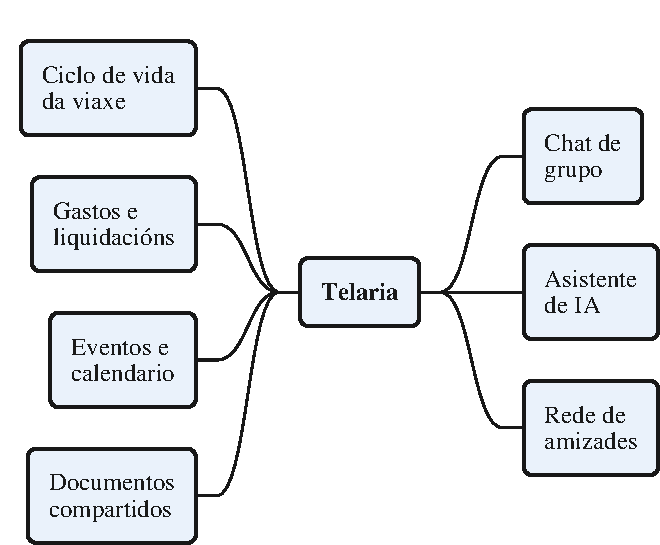
\includegraphics[width=0.80\textwidth]{diagrams/funcionalidades-telaria.pdf}
  \caption{Funcionalidades principais de Telaria.}
  \label{fig:funcionalidades-telaria}
\end{figure}

\textbf{Ciclo de vida da viaxe.} A viaxe é a unidade central arredor da que se organiza
todo o demais. Un usuario crea unha viaxe e convida a outras persoas, que poden
incorporarse por invitación directa, solicitando o acceso ou escaneando un código QR;
calquera membro pode abandonala e xestionar as solicitudes pendentes.

\textbf{Gastos e liquidacións.} Cada membro pode rexistrar os gastos que paga, indicando
os beneficiarios e unha categoría (aloxamento, transporte, comida, etc.). A partir deses
rexistros, o módulo calcula automaticamente o balance de cada persoa e propón un conxunto
de liquidacións aplicando un algoritmo de minimización de débedas, de xeito que o número
de transferencias necesarias para saldar todos os saldos sexa o mínimo posible. As
liquidacións xa realizadas consérvanse nun historial.

\textbf{Eventos e calendario.} O grupo constrúe un itinerario común sobre un calendario
compartido. Cada evento pode ter data, hora, duración e unha localización xeográfica,
que se pode escoller buscando un enderezo ou seleccionándoo directamente nun mapa
interactivo.

\textbf{Documentos compartidos.} A viaxe dispón dun repositorio de documentos relevantes
(reservas, billetes, fotos, etc.) que calquera membro pode subir, descargar ou eliminar.
Para os documentos de imaxe xérase de forma asíncrona unha miniatura de previsualización,
de modo que a listaxe se mostre con axilidade sen descargar os ficheiros orixinais.

\textbf{Chat de grupo.} Cada viaxe inclúe unha sala de conversa propia para a
coordinación entre os membros, con entrega de mensaxes en tempo real e aviso de mensaxes
sen ler. As mensaxes son almacenadas no servidor durante 30 días
e despois son eliminadas automaticamente.

\textbf{Asistente de intelixencia artificial.} Cada viaxe conta cun asistente
conversacional que axuda na planificación e responde consultas. Mantén un historial de
conversa independente por viaxe e por usuario, de modo que o contexto se preserve entre sesións.
Por razóns de rendemento do modelo local, este só recibe como contexto as últimas 5 mensaxes do
chat (ademais do contexto da viaxe),
se ben as demais mensaxes quedan almacenadas e dispoñibles para consulta. O historial completo de conversa mantense durante 30 días.

\textbf{Rede de amizades e xestión de conta.} De maneira complementaria, a plataforma
ofrece unha rede de amizades entre usuarios: calquera usuario pode engadir outros como
amigos e, a partir de aí, convidalos ás súas viaxes de forma máis áxil que mediante o
identificador ou o código QR. Esta funcionalidade non altera o modelo colaborativo
descrito, senón que actúa como atallo para os usuarios habituais. Cada usuario xestiona
ademais o seu propio perfil (nome, correo, avatar e contrasinal) e pode eliminar a súa
conta, operación que require a confirmación do contrasinal. A aplicación está dispoñible
en tres idiomas (galego, español e inglés) e ofrece temas de aparencia clara e escura.

Como obxectivos técnicos, o proxecto busca aplicar unha arquitectura
\textit{API-first} e tecnoloxías multiplataforma modernas, de xeito que a solución
sexa funcional tanto en iOS como en Android dende unha única base de código.

\section{Relación da documentación que conforma a memoria}

\begin{tabularx}{\textwidth}{@{}lX@{}}
  \toprule
  \textbf{Sección} & \textbf{Contido} \\
  \midrule
  Resumo                            & Breve resumo das principais contribucións do traballo. \\[4pt]
  Introdución                       & Obxectivos xerais, descrición do sistema e tecnoloxías e arquitecturas empregadas. \\[4pt]
  Especificación de Requisitos      & Requisitos funcionais e non funcionais, interfaces con outros sistemas e información que o sistema debe almacenar. \\[4pt]
  Deseño                            & Arquitectura do sistema, división en compoñentes e comunicación entre eles. Equipamento hardware e software empregado. \\[4pt]
  Probas                            & Plan de probas con evidencias que verifican a funcionalidade e corrección global do sistema. Resultados acadados. \\[4pt]
  Conclusións e Posibles Ampliacións & Grao de cumprimento dos obxectivos e posibles vías de mellora futura. \\[4pt]
  Bibliografía                      & Lista completa de referencias citadas no texto. \\[4pt]
  Manuais Técnicos                  & Documentación para desenvolvedores: código fonte, recursos necesarios e operacións de modificación e proba. \\[4pt]
  Manuais de Usuario                & Documentación autocontida para usuarios finais: instalación, uso, configuración e mensaxes de erro. \\
  \bottomrule
\end{tabularx}

\section{Información adicional de interese}

\subsubsection*{Arquitectura API-first con OpenAPI}

O deseño do sistema parte da especificación da API antes de calquera implementación.
Isto establece un contrato explícito e verificable entre frontend e backend, permite
xerar documentación interactiva de forma automática (Swagger UI)~\cite{openapi} e facilita o
desenvolvemento en paralelo de ambos os extremos.

\subsubsection*{React Native e Expo}

O frontend está desenvolvido con React Native~\cite{reactnative}, o que permite compartir a mesma base
de código para iOS e Android. Expo~\cite{expo} engade sobre React Native unha capa de utilidades
que simplifica a xestión de dependencias nativas, o proceso de compilación e a
distribución da aplicación, reducindo a complexidade de configuración do proxecto.

\subsubsection*{Spring Boot}

O backend emprega Spring Boot~\cite{springboot} pola súa madurez e polo seu ecosistema integrado: Spring
MVC para a capa REST, Spring Data JPA para a persistencia, Spring Security para a
autenticación e autorización, e integración directa con bibliotecas de xeración de
documentación OpenAPI.

\subsubsection*{Autenticación baseada en JWT}

O mecanismo de autenticación utiliza dous tokens complementarios. O \textit{access
token}, de tipo JWT~\cite{rfc7519} e vida curta, inclúese en cada petición á API e permite verificar
a identidade do usuario sen consultar a base de datos. O \textit{refresh token}, de
tipo opaco e almacenado no servidor, emprégase exclusivamente para renovar o
\textit{access token} e pode invalidarse explicitamente no peche de sesión.

\subsubsection*{Ollama}

O asistente conversacional funciona sobre Ollama~\cite{ollama}, un motor de inferencia local de
modelos de linguaxe grande. A execución local elimina a dependencia de servizos
externos de pago, preserva a privacidade dos datos dos usuarios e ofrece latencias
predecibles independentes de terceiros.

\subsubsection*{Almacenamento de obxectos compatible con S3}

Os documentos compartidos almacénanse nun servizo compatible co protocolo S3~\cite{minio}. A
elección deste estándar garante a independencia do provedor e aproveita o soporte
nativo dispoñible en Spring Boot mediante o AWS SDK. Para os documentos de imaxe,
ao confirmar a subida lánzase de forma asíncrona mediante un virtual thread,
fóra da ruta de petición, a xeración dunha miniatura de previsualización reducida
que se mostrará na listaxe sen necesidade de descargar o ficheiro orixinal.

\subsubsection*{PostgreSQL}

A base de datos relacional escollida é PostgreSQL~\cite{postgresql}, pola súa robustez, polo seu soporte
nativo para UUID e tipos de data con fuso horario, e pola súa excelente integración
con Spring Data JPA.

\subsubsection*{Podman}

O despregamento dos servizos realízase mediante contedores OCI xestionados con Podman~\cite{podman}.
A diferenza de Docker, Podman opera sen un daemon centralizado e permite executar os
contedores sen privilexios de superusuario (\textit{rootless}), o que mellora o
illamento de seguridade do entorno de execución.

\subsubsection*{Tarefas periódicas}

Existen tres tarefas programadas de mantemento. A primeira percorre periodicamente os
documentos de imaxe sen miniatura como rede de seguridade para os casos nos que a
xeración inmediata fallase. A segunda reconcilia o estado dos documentos non confirmados
co almacén de obxectos, recuperando os que chegaron ao almacén sen ser confirmados e
eliminando os que non chegaron. A terceira elimina mensaxes de chat (tanto grupais como
do asistente de IA) que superan os 30 días de antigüidade. Estas tarefas evitan o
crecemento indefinido da base de datos e do almacenamento de obxectos.
